\chapter{Azimuthal Correlations of Non-Photonic Electrons to Hadrons}

We will now investigate the correlations of triggered non-photonic electrons to hadrons in $\auau$ and $\pp$ collisions at 200 GeV. Hard processes in these collisions will produce back to back jets in the azimuthal angle $\phi$. We search for potential modification of the jet in $Au+Au$ collisions compared to $\pp$. 

\section{Overview of Constructing the NPE-hadron Correlation}

Several steps are needed to produce the NPE-h correlation. The trigger particle electrons are identified by the procedure described in the previous chapter. The nonuniform acceptance of detector results in false correlations which are not a result of the underlying physics. This is corrected in two ways, the $\phi$ distribution of all particles in flattened and then the correlations from mixed events are calculated and then a weighting is determined so as to flatten these as well.

In correlations from $Au+Au$ collisions there is an underlying background correlation from the flow of the both the trigger electron and the associated hadron. In this analysis we only consider the second order harmonic of flow, $v_{2}$. For hadrons, $v_{2}$ is very accurately measured across a wide range centralities and $p_{T}$. For non-photonic electrons, the measurements of $v_{2}$ are not so precise, thus we can only estimate its contribution to the background. This uncertainty will be reflected in the analysis of systematic error.

We will also look at the dependence of the correlation on the angle between the triggered electron and the event plane. A dependence on this angle could point to path length dependence on the jet suppression in QGP.

\section{Acceptance Corrections}

The STAR detector give full $2\pi$ azimuthal coverage, however there are still regions of the detector which have noticeably poorer efficiency. This causes an uneven azimuthal acceptance which in turn lead to spurious correlations between detected particles. To correct this we need to apply a weighting to each track depending on where it is in the detector. 

\subsection{Single Particle $\phi$-weighting}

We begin by correcting for the single particle acceptance in $\phi$. The boundaries between sectors produce regions of lower efficiency, also in Run11 one sector of the TPC had noticeably lower efficiency than the rest. These effects are both shown in Figure~\ref{fig:PhiDistAllTracks}.  

\begin{figure}[htbp]
\begin{center}
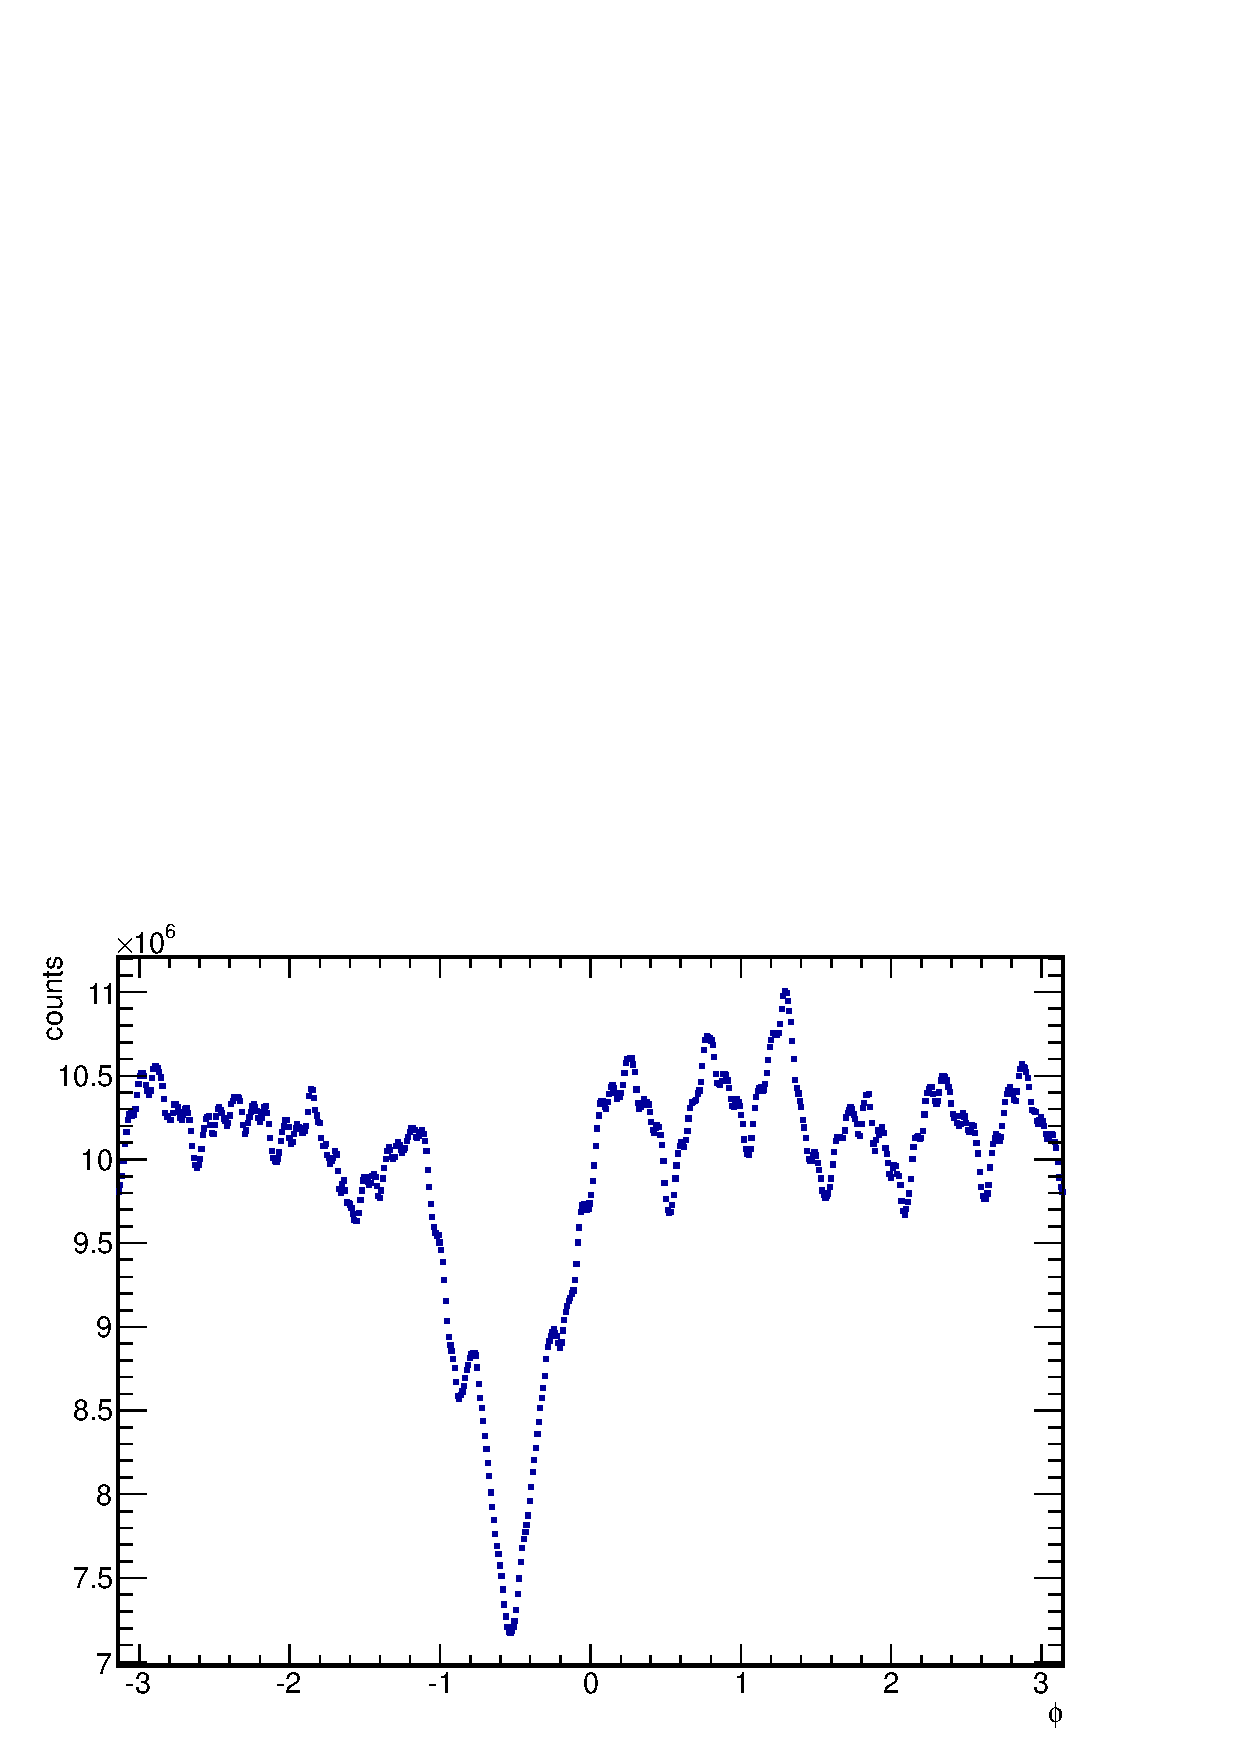
\includegraphics[scale=.8]{Plots/Correlations/Phi_All.pdf}
\end{center}
\caption[Phi distribution for all tracks in TPC.]{The azimuthal angular distribution of all tracks in Run11 $Au+Au$ collisions at 200 GeV. Periodic bumps can be seen from the sector boundaries, as well as a dip in the poorly performing sector.}
\label{fig:PhiDistAllTracks}
\end{figure}

The dependence of the acceptance on $\phi$ however is not the same for all tracks. Whether a track crosses a sector boundary or passes through the dead sector will depend on that particular track's geometry. Tracks at low $\pt$ curve more in the magnetic field and thus the effects of these lower efficiency areas apply to wider regions in track $\phi$. The dependence of acceptance on $\pt$ is shown in Figure~\ref{fig:PtDependPhi}. At low $\pt$ the dependence is especially strong thus for $\pt \leq 1$ GeV/c we divide tracks into $\pt$ bins of .1 GeV/c, which is near the limit of the momentum resolution of the TPC. Above 1 GeV/c the tracks are roughly straight so the effects on acceptance from the sector boundaries and dead sector are consistent bin-to-bin up to arbitrarily large $\pt$.

\begin{figure}[htbp]
\begin{center}
\includegraphics[scale=.8]{Plots/Placeholder.pdf}
\end{center}
\caption[$\pt$ dependence of $\phi$ acceptance]{$\phi$ distributions for single particles in different $\pt$ bins. Strong $\pt$ dependence is seen especially below 1 GeV/c due to the different track geometries.}
\label{fig:PtDependPhi}
\end{figure}

While the dependence of acceptance on track $\pt$ is by far the largest effect, we still further subdivide the tracks to make acceptance corrections. It is possible for the acceptance to depend on $\eta$, and we are especially concerned with edge effects when  $|\eta| \sim 1$, thus we divide into 4 even bins in pseudorapidity ranging from -1 to 1.

Likewise we account for dependence on the event vertex (in both $\pp$ and $\auau$) and multiplicity (only for $\auau$) by dividing into bins of vertex-z and centrality. For the centrality bin divisions, all centrality bins from $30\%-80\%$ are taken together since in the peripheral bins the statistics are too low to get a reliable acceptance correction.

Finally, since the tracks in the TPC are curved, there will be a dependence on which direction the track curves. For example, two particles may start on opposite sides of a sector boundary separated by some distance in $\phi$ but both may cross the boundary if they curve in opposite directions. So we need to take separate weightings based on the product of the magnetic field and the particle's charge, $B \cdot q$. 

After calculating the single $\phi$ correction we apply it to each track in the analysis whenever we calculate event planes or 2-particle correlations. Since some areas of the detector have very low efficiencies they can introduce huge weights for a small number of particles. This can destabilize results, so we cap the weight an individual particle can get at 5.0.

\subsection{Mixed Event Background}

To further correct for nonuniformities is detector acceptance we use a mixed event weighting. In an ideal detector the correlations of trigger particles to associated hadrons from a different event should be flat, however acceptance effects will result in nonphysical correlations which need to be removed. 

Similar to the single particle corrections we divide the mixed event corrections into bins to account for various systematic differences. In mixed event we bin according to associated particle $\pt$, triggered particle $\pt$, centrality, vertex z position, and $\eta$. As in single particle corrections, the most extreme bin to bin variationsoccur between the low associated $\pt$ bins.   

\section{Background from Flow}

\subsection{Measurements of Flow}

The motivations behind two-particle correlation studies are typically the investigation of jet modification in QGP and the response of the medium to jets. But even in the absence of jets we still expect to see some correlation within events from flow. The azimuthal anisotropy resulting from the second order flow harmonic, $v_2$, of both the trigger and associated particles produces a background shape with the form:
\begin{equation}\label{eq:v2background}
 B[1 + v^{trig}_{2}v^{asso}_{2} cos(2\Delta\phi)] 
\end{equation}

where $B$ is an overall constant factor. Higher order harmonics $v_3$, $v_4$, etc. can also contribute to the background. Large $v_3$ in particular is a potential explanation for some of the results in dihadron correlations, but these effects are not considered for this analysis. 

Hadron $v_2$ has been measured to high precision in a wide range of $\pt$ bins at STAR. Figure~\ref{fig:STARHadv2} shows the results of STAR $v_2$ measurements using an event plane method and illustrates the general depedence on $\pt$ and centrality. To calculate the hadron $v_2$ we extrapolate the $v_2$ measurement to the center of the associated hadron $\pt$ bin. Then when looking at correlations across multiple hadron $\pt$ bins we use the weighted average of $v_2$ based on the number of hadrons in each $\pt$ bin.

\begin{figure}[htbp]
\begin{center}
\includegraphics[scale=.8]{Plots/Placeholder.pdf}
\end{center}
\caption[STAR measured hadron $v_2$]{Measured $v_2$ values for hadrons across a range of $\pt$ and centralities.}
\label{fig:STARHadv2}
\end{figure}

Measurements of electron $v_2$ at STAR have shown that non-photonic electrons also have large elliptic flow. Because of limited statistics electron $v_2$ is measured in much larger $\pt$ and centrality bins. Various measurements of NPE $v_2$ are seen in Figure~\ref{fig:STARNPEv2}, showing that they tend to fall in a range between .05 and .15 depending on the measurement procedure. For this analysis we assume that NPE $v_2$ is .1 in all bins, we then vary the NPE $v_2$ between .05 and .15 and take the difference in final correlations as a systematic error. 

\begin{figure}[htbp]
\begin{center}
\includegraphics[scale=.8]{Plots/Placeholder.pdf}
\end{center}
\caption[STAR NPE $v_2$]{Various measurements of NPE $v_2$ in STAR. Going forward we assume .1 to be the value for NPE $v_2$ in all bins.}
\label{fig:STARNPEv2}
\end{figure}

\subsection{Background Normalization}

Knowing the values of $v_2$ for hadrons and non-photonic electrons, we then need to determine the overall normalization constant $B$ as in Equation~\ref{eq:v2background}. There are two simple ways of estimating this, both relying on the assumption that the jet like contributions to the azimuthal correlation are concentrated in peaks around 0 and $\pi$, and that any remaining correlations there are the result of the underlying $v_2$ background. 

In one case we can simply pick a point between the near and away sides and then set $B$ so that the overall yield of particles above background at that point is 0. This point is typically taken to be around 1 radian and thus this method is called the zero yield at 1 (ZYA1) normalization. Although when we implent ZYA1 normalization we take the lowest absolute yield of the 3 points closest to 1 radian. Alternatively we can instead pick the point in the raw correlation with lowest value and normalize so that that point produces zero yield. This is the zero yield at minimum (ZYAM) method. These methods tend to coincide in practice and unless otherwise noted we use ZYAM normalization. There is another technique called absolute background subtraction used by PHENIX in their NPE-hadron correlation measurement but we do not use this method. 

When using ZYAM or ZYA1 normalization our background subtracted yield can be very suceptible to downward fluctuations of points causing an abnormally high yield. To account for this we also look at the effect of normalizing to the next highest point in the correlation. We then compare the values of $B$ that we get and then quote the difference as the systematic error of background normalization.

\section{Correlations in Au+Au}

We will now look at putting together the results of the previous sections and creating the NPE-h correlation in Au+Au collisions. We will then discuss the results in Au+Au before moving on to p+p and event plane dependent correlations.

\subsection{Constructing the NPE-hadron correlation}

Now with azimuthal electron-hadron correlation functions we look at how we create the NPE-h correlation. The definition of the NPE-h correlation is:

\begin{equation}\label{eq:NPEhdef}
 \frac{dN_{NPE-h}}{d\Delta\phi} = \frac{dN_{semi}}{d\Delta\phi} - \left(\frac{1}{\epsilon_{\gamma}} - 1\right)\frac{dN_{NPE-photonic}}{d\Delta\phi} + \frac{dN_{same}}{d\Delta\phi}   
\end{equation} 

\section{Correlations in p+p}

\section{Event-Plane Dependent Correlations}

\section{Event Plane Reconstruction}

